%\section{Mining \acs{VCS} Event Data}
\label{sec:bpm2015concept}
In the following, we first formalize the notions encountered in the project mining setting. Then we develop an approach to acquire a hierarchical overview on the project from a repository perspective.

\subsection{Preliminaries}
\glspl{vcs} are used in projects to ensure reliable collaboration. We build our approach on \gls{vcs}. Typically, the workflow in \gls{vcs} is that people work on files (e.g., text, source code, spread sheets) and commit them to the central repository. Project participants comment on their commits so that other participants can better understand the nature of the changes to the files.

Let \Files be the universe of files. Files are organized in a file tree. Therefore, each file $\file \in \Files$ has one parent file. The only file without a parent file is the root file. We capture this information in the parent relation $\parent : \Files \times \Files$. For example, let $\file_p \in \Files$ be the parent of file $\file_c \in \Files$, then $(\file_p, \file_c) \in \parent$.
The transitive closure on the parent files is given by the function $\ancestor : \Files \rightarrow 2^{\Files}$ that returns the set of files along the path to the root.

When project members did a certain amount of work and want to save their current progress, they commit the changes to the \gls{vcs}.
We define changes on files as the events of interest on the lowest granularity.
\begin{definition}[Event] \label{def:bpm2015events}
Let $\Events$ %  = \Files \times \ChangeOperations \times \Timestamps \times \Comments \times \ChangedAmount$
be the set of events. An event $\event \in \Events$ is a four-tuple $(\file, \changeOperation, \timestamp, \comment)$, where
\begin{compactitem}
  \item $\file \in \Files$ is the affected file of the event.
  \item $\changeOperation \in \ChangeOperations =\lbrace\added$, $\modified$, $\deleted \rbrace$ is the change operation on the file with obvious meaning.
  \item $\timestamp \in \Timestamps = \mathbb{N}_0$ represents a unix time stamp marking the time of the event occurrence.
  \item $\comment \in \Sigma^*$ is a comment in natural language text.
%  \item $\changedAmount \in \ChangedAmount$ is the absolute number of changed bytes in comparison to the previous version of the file.
\end{compactitem}
% Let $\ChangeOperations = \lbrace \added$, $\modified$, $\deleted \rbrace$ be the set of change operations on files, \Timestamps represent unix time stamps, and $\Comments \subseteq \Sigma^*$ be comments in natural language text.
% Events $\event \in \Events$ are tuples of the form .
% \todo{TODO: decide, if we need weights on how much of the files changed.
% Also: what about resources?}
%$\file \in \Files$ is a file, $\changeOperation \in \ChangeOperations$ is a change operation, $\timestamp \in \Timestamps$ is a timestamp, and $\comment \subset \Sigma^*$ is a comment in natural language text.
\end{definition}

For events $\event = (\file, \changeOperation, \timestamp, \comment%, \changedAmount
)$ we overload $\file, \changeOperation, \timestamp$, and $\comment$
%,$ and $\changedAmount$ 
to be used as accessor functions. For example, \file is the function $\file : \Events \rightarrow \Files$ mapping an event to its affected file.

Project participants can commit a number of changes to different files at one step. Therefore, we define the notion of commits as follows.
%\todo{Maybe instead use a reduction of an event like $\event_{|\timestamp}$}

\begin{definition}[Commit]
A commit $\commit$ is a set of events sharing the same time stamp and comment, i.e., $\forall \event, \event' \in \commit: \timestamp(\event) = \timestamp(\event') \wedge \comment(\event) = \comment(\event')$. Additionally, each event in a commit affects different files, i.e., $\forall \event, \event' \in \commit : \event \neq \event' \rightarrow \file(\event) \neq \file(\event')$.
\end{definition}
%\todo{Decide: Do we need the definition Commits at all?}

Usually, it is in the hands of project participants, when they decide to commit changes to the \gls{vcs}. In the extreme case, there could be only a single commit made in a project that adds all files to the repository.
Note that this extreme practice would render the use of a \gls{vcs} obsolete. On the contrary, it is common practice to regularly perform commits in order to securely store work progress and to reduce the chance of conflicts~\citep{pilato2008version,Hou2014}. Conflicts occur, when another participant committed changes to a file that is being committed and can cause extra work.
Based on these insights, we make the assumption that commits are regularly made during work.

Projects are decomposed into work packages. We assume a hierarchical work package structure of a project, such that a work package can have sub work packages. Further, the amount of work in a single work package need not be done in one single time span, but it can be split into several activities. Activities have a start and end time, and subsequent activities can have idle periods in between. Thus, we define projects as follows.
\begin{definition}[Project]\label{def:bpm2015project}
A project \Project is a tuple $(\WorkPackages, \Structure, \Activities, \startTimeFunction, \finishTimeFunction, \MappingFunction)$, where
\begin{compactitem}
  \item $\WorkPackages$ is the set of work packages in the project.
  \item $\Structure \subseteq \WorkPackages \times \WorkPackages$ is the relation that hierarchically decomposes work packages into a tree structure.
  \item $\Activities$ is the set of activities that are conducted in the work packages.
  \item $\startTimeFunction : \Activities \rightarrow \Timestamps$ is the function that assigns a start time to activities. Activities are ordered by their start times.
  \item $\finishTimeFunction : \Activities \rightarrow \Timestamps$ is the function that assigns an end time to activities.
  \item $\MappingFunction : \Activities \rightarrow \WorkPackages$ is the mapping function that maps activities to their corresponding work packages.
\end{compactitem}
\end{definition}

Note that this definition reflects an activity centric view on projects. The definition deliberately omits further dimensions, e.g., costs, resources, risks. The idea is not to capture projects in every detail, but to focus on the work packages of a project to obtain an overview of the work that is being done. %\todo{Question: do we want a full-blown definition on projects? with risks, resources, milestones, stakeholders, \ldots?}
We are interested in when work has been started in a work package, and when work packages have been done. This information can be derived from the activities associated to the workpackages. An obvious assumption is that the work package starts with its first activity, and ends when its last activity is completed.

Based on these notions, we can define the task of \emph{project discovery} as reconstructing the project \Project from a set of low level event data \Events.
In the following, we present an approach to this problem.

% \begin{definition}[Project mining]
% 	Given a set of events \Events, the objective of project mining is to identify:
% 	\begin{compactitem}
% 		\item the set of work packages \WorkPackages in the project.
% 		\item the start \startTimeFunction, and end \finishTimeFunction of the workpackages in \WorkPackages.
% 		\item the hierarchical relation \Structure between work packages.
% 		\item the mapping function \MappingFunction that assigns assigns events to a work package.
% 	\end{compactitem}
% \end{definition}


% Inital definition which we have to align to the current \\
% A commit is a set of change operations. $\commit \equiv \lbrace c \in \changeOperation \rbrace \times \comment$ \\
% A change operation is a set of triples $\changeOperation \equiv \lbrace F, W, O \rbrace $ where $F, W, O$ are respectively the file, the weight (how much a change affected the file), and the operation type ($O={modified,added,deleted}$)\\
% Upon the above sets we can define functions such as a modification function (that, for instance, maps the set of files to their weight), or distance(f1, f2) (but for the moment we don't use it).\\ \vfill

% After the last discussion I identified the following concepts to be formalized. So basically we would need to align the initial definition to was follows.
%
% Definitions: \\
% \begin{definition}[Event]
% Event: something that happens at some point in time. Generally in the past. (Primitive concept: can't be derived from any other concepts? Can it be defined?!)
% Event data: data regarding events. An event over a dataset A is the minimum amount of modification made to the minimum part of A at some point in time. i.e. the smallest possible change.
% \end{definition}
%
% \begin{definition}[Project]
% D2. Project (hierarchy) \\
% a project has a hierarchy. It is a set of event streams. An event stream is an object of the hierarchical structure. (that relates to events).
% \end{definition}
%
% We define a mapping function $f$ from the set of events to objects which is:
% \begin{itemize}
% \item surjective and not injective (i.e. every element in the codomain has a corresponding element if the domain, and it doesn't hold that for two different elements $a, b$ of the domain there exist two different mappings $f(a), f(b)$ in the codomain.
% \item total
% \end{itemize}
%
% Function $f$ partitions the set of events...
% \begin{definition}[Commit]
% A commit is a "bundle" of events.\\
% \end{definition}

% \begin{definition}[Drill]
% Here we formally define the agglomeration feature. We can drill-up and drill-down on the data. E.g. show grouped events for folders at different levels.
% \end{definition}

\subsection{Time Perspective Discovery}\label{sec:subsec:discovery_technique}
\begin{figure}[b]
\centering
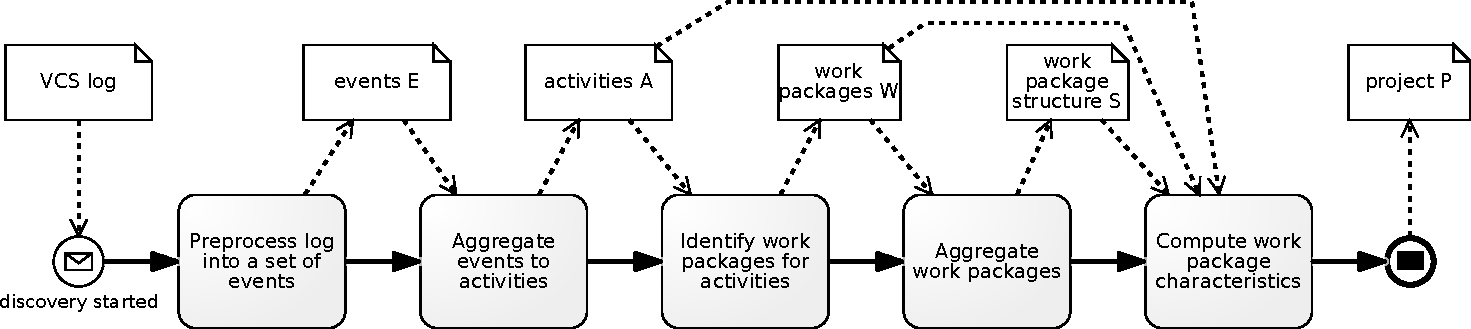
\includegraphics[width=\textwidth]{bpm2015/imgs/Project_discovery}
\caption{Project discovery technique overview as BPMN process model.}
\label{fig:project_discovery_technique}
\end{figure}
For project discovery from the \gls{vcs} commit history, we need to identify activities that are performed, associate the activities to work packages and recreate the work package structure of the project.
Our aim is to create a hierarchical model that provides an overview of the project work.
Therefore, we have to identify the start and end times of activities and of work packages before we can visualize the project work. The input to the technique is the log that is stored in the \gls{vcs}. The challenge is that the raw log only records commits on the file system level and information on activity level is missing. However, we can deduce activity information from events based on the following assumptions.

\begin{itemize}
  \item \textbf{A1: Meaningful file tree structure.} The file tree structure in a project represents its work package structure. That is, the knowledge workers organize their work in a file hierarchy that reflects the project structure.
  \item \textbf{A2: Local changes.} Activities in a work package affect only files of the work package folder, or in the corresponding sub-tree in the file tree structure.
  \item \textbf{A3: Frequent commits.} Commits to the \gls{vcs} are regularly performed, when conducting work in an activity.
\end{itemize}

Note that assumption A1 can be seen as a strong assumption on the file tree structure. Nevertheless, we argue that even if A1 is not entirely met, the aggregation of work information on the file tree hierarchy provides a valuable view on the project.
Figure~\ref{fig:project_discovery_technique} shows the different steps of the technique. We describe each of them in detail.

\subsubsection*{Step 1: Preprocessing.} The first step is to transform raw logs of version control systems (which might be grouped by commits) into a list of events as specified in Definition~\ref{def:bpm2015events}. This step is easily done by replicating the information on commit level to be contained in the events. The output is a set of events \Events.

\subsubsection*{Step 2: Aggregating events to activities.}
Given the set of events \Events that we gathered from a version control system, the next step is to identify the activities to which the events belong. Note that we do not know the activities of the project in advance, but need to infer them based on the events. Each event affects a single file in the file hierarchy.

\begin{figure}
\centering
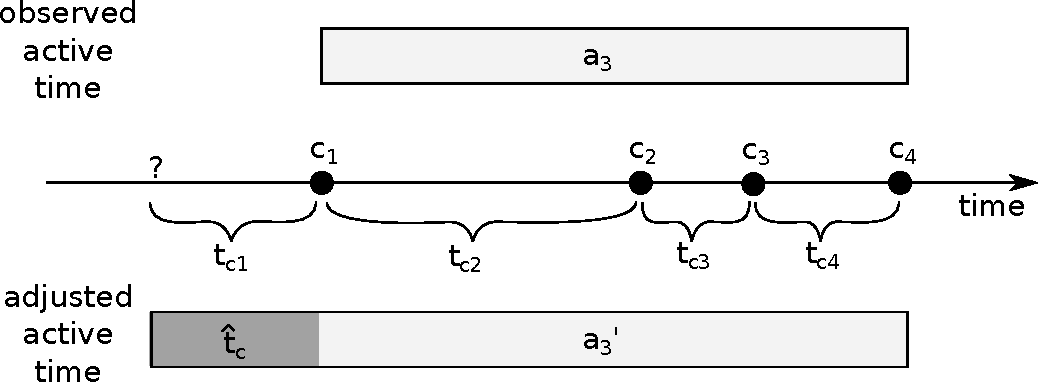
\includegraphics[width=.7\textwidth]{bpm2015/imgs/activity_adjustment}
\caption{Adjustment of activity start time \startTimeFunction. }
\label{fig:activity_adjustment}
\end{figure}

Based on assumption A2, we are interested in activities conducted in a work package, that is, we filter for the events that are contained in the given file or its children. For every file $\file$ of interest, we select the set of events affecting the file or its children as $\Events_{\file} = \lbrace \event \in \Events \mid \file = \file(\event) \vee \file \in \ancestor(\file(\event))  \rbrace$. The task is then to find the activities which emitted the set of events $\Events_{\file}$. We rely on assumption A3, which states that during an activity, we expect multiple commits. Assumption A3 allows us to conclude that if we do not observe commits for a longer period of time, there is no activity being performed in the work package.

%To derive coarse grained activities from low level events, clustering techniques~\cite{Berkhin2006ClusteringSurvey}, or abstraction functions~\cite{baier2014bridging} can be used.
%Former assume that a distance function measures the distance between events, and partitions the set of events into groups. Well-known examples are the k-means clustering~\cite{Berkhin2006ClusteringSurvey}, or hierarchical agglomerative clustering.
To this end, we adopt the abstraction technique by \citep{baier2014bridging} and allow the domain expert to formulate rules for aggregating events to activities based on boundary conditions. Assuming that people frequently commit their progress (A3), we can specify a boundary condition based on the temporal distance to previous events. For example, we can specify that a time period of seven days without a commit is a boundary condition. %But also other boundary conditions can be selected, e.g., based on resources.
As the result, we obtain the mapping from events to these activities, which we call $\eventMapping_{\file} : \Events_{\file} \rightarrow \Activities_{\file}$ in the remainder of the paper. The set of discovered activities identified for the work package based on given boundary conditions is then $\Activities_{\file} = \lbrace \activity \mid \event \in \Events_{\file}, \eventMapping_{\file}(\event) = \activity \rbrace$. We also define the inverse mapping, that is, the mapping from an activity to its events as $\eventMapping_{\file}^{-1} : \Activities_{\file} \rightarrow 2^{\Events_{\file}}$.

With the events mapped to activities, we need to find the temporal boundaries of the target activities. That is, we define the functions $\startTimeFunction$ and $\finishTimeFunction$ for each activity. The challenge here is that we do not know when an activity actually started, because the start of the activity is not recorded in the \gls{vcs}. We can only observe the time of the first commit in that activity, but commits usually mark progress of an already running activity.

To address the challenge of missing start times, we impute the missing start time by prepending the expected active time $\expectedActiveTime$ before a commit, as illustrated by Figure~\ref{fig:activity_adjustment}. This notion assumes that project participants commit their work progress after a certain amount of time. However, we cannot compute \expectedActiveTime by looking at the average commit rate in a work package, because this average is based on busy periods and idle periods. We need to factor out the idle periods in the computation of this measure.
%Therefore, we use the following formula.
%Let $\file$ be a file in the file tree that represents a work package, and let $\Events_{\file}$ be the corresponding events for all the children of $\file$. Let further $\Activities$ be the activities identified for the work package based on given boundary conditions.
We know the end time of the activities, as the last commit marks the completion of work. Therefore, each activity \activity based on given boundary conditions has the associated end time $\finishTimeFunction(\activity) = \max(\lbrace \timestamp(\event) \mid \event \in \eventMapping_{\file}^{-1}(\activity)  \rbrace)$. Further, we write the first event's timestamp of an activity as the function $\startTimeFunction'(\activity) = \min(\lbrace \timestamp(\event) \mid \event \in \eventMapping_{\file}^{-1}(\activity)  \rbrace)$.
Then, we define $\numCommits:\Activities_{\file} \rightarrow \naturalNumbers$ as the number of commits in one activity, formally $\numCommits(a)=|\lbrace \commit \mid \event \in \commit \wedge \eventMapping_{\file}(\event)=a\rbrace |$.

With this information the expected active time between commits \expectedActiveTime is given as follows.

\begin{equation}
	\expectedActiveTime = \frac{\sum_{\activity \in \Activities_{\file}} \left(\finishTimeFunction(a) - \startTimeFunction'(a)\right)}{\sum_{\activity \in \Activities_{\file}} (\numCommits(\activity)-1) }
\end{equation}

We assume that there is at least one activity spanning over at least two commits, i.e., $\exists \activity \in \Activities_{\file} \mid \numCommits(\activity) > 1 $. Translated to our boundary condition, this assumption is that there is at least one week in each work package, in which there were at least two commits made. Otherwise, we set $\expectedActiveTime$ to 0 for the current file \file due to lack of information.

Given the expected active time between commits $\expectedActiveTime$, we can finally adjust the start time of each activity. Therefore, we set the associated start time for each activity as $\startTimeFunction(\activity) = \startTimeFunction'(\activity) - \expectedActiveTime$. That is, we subtract the expected active time from the first commit's timestamp.

We apply Step 2 to all files $\file$ in the file tree to get $\Activities_\file$. For the remainder of this paper, we define the function $\fileToActivity : \Activities \rightarrow \Files$ that contains the mapping information of the discovered activities to their originating files. Finally, we set the activities \Activities in the project to be the union of the activity sets per file $\bigcup_{\file \in \Files} \Activities_\file$.

% \begin{definition}[Abstraction Function]
% Formally, we rely on an abstraction function $\abstractionFunction : 2^{\Events} \rightarrow 2^\Activities$ that maps a set of events to a set of activities.
% \end{definition}
%
% The abstraction function \abstractionFunction operates on a set of events


\subsubsection*{Steps 3 and 4: Mapping activities to work packages and aggregating.}
Once activities have been identified, we want to climb to the next abstraction layer: the work packages. Assumption A1 allows us to specify a one-to-one mapping $\kappa : \Files \rightarrow \WorkPackages$ between files in the file tree structure and work packages. More precisely, we construct the set of work packages $\WorkPackages$ isomorphic to the set of files $\Files$, such that the $\parent$ relation is preserved in the work package structure \Structure relationship. %This way, we assign the discovered activities of a selected file $\file'$ to the work package corresponding to $\file'$.

The mapping $\MappingFunction$ of activities to work packages is simply $\MappingFunction(\activity) = \kappa (\fileToActivity(\activity))$. That is, the corresponding work package of the activity that was discovered for a file.
%The aggregation of work packages is done according to the hierarchy obtained from the file tree structure.
In this way, we provide an activity based view on work packages, and we can aggregate on each level in the file system to see active periods of the corresponding hierarchy level.


\subsubsection*{Step 5: Computing work package characteristics.} In this final step, we compute measures of interest for the discovered work packages. First, we obtain the temporal boundaries of a work package by the functions $\startTimeFunction$ and $\finishTimeFunction$ of the associated activities.

Let $\MappingFunction^{-1} : \WorkPackages \rightarrow 2^{\Activities}$ be the inverse of the mapping function $\MappingFunction$ of the project.
The start and end time of a work package ($\startTimeFunction_{\WorkPackages}$ and $\finishTimeFunction_{\WorkPackages}$) are functions from work packages to timestamps. The start time is defined as $\startTimeFunction_{\WorkPackages}(\workPackage) = \min(\lbrace \startTimeFunction(\activity) \mid \activity \in \MappingFunction^{-1}(\workPackage)\rbrace )$, and the end time function of work packages $\finishTimeFunction_{\WorkPackages}$ is analogously defined using the maximum of the end times $\finishTimeFunction(\activity)$ of the activities.
We call the duration of a work package $\durationOfWorkPackage$ that is the difference between $\finishTimeFunction_{\WorkPackages}$ and $\startTimeFunction_{\WorkPackages}$.

Moreover, we are interested in the ratio of active working periods (i.e., the time spans of activities) to the total work package duration. This quantity helps to estimate the average work intensity in a work package.

\begin{definition}[Coverage]
The coverage \coverage of work packages by activities is a function $\coverage : \WorkPackages \rightarrow [0,1]$ and is defined as follows.
\begin{equation}
\coverage(\workPackage) = \frac{\sum_{\activity \in \MappingFunction^{-1}(\workPackage)}  \left(\finishTimeFunction(a) - \startTimeFunction(a)\right)}{\durationOfWorkPackage(\workPackage)}
\end{equation}

\end{definition}

With this final step, we lifted the information hidden in low level events to a high-level Gantt chart perspective, with which project managers are familiar. In the following, we compare our technique to existing process mining approaches.


% Here, we present a first approach to project mining that serves to offer a rough estimation on the work packages and their structure in a project.
% The proposed approach in this paper builds on the assumption that the file structure in the project repository is meaningful.
%
% %We acknowledge that this assumption might not be valid in all cases, but we shall demonstrate the usefulness of the approach
%
% Based on this assumption, the main task of project mining is to identify activities that are performed and map them to the work packages of the project.
%
%
%
% The approach is based on the general assumption that there is a \emph{distance} between events and we can algorithmically measure it.



% Technique: \\
%
% Algorithm (from VCS to project) \\
% \begin{verbatim}
% pseudocode of the algorithm
% \end{verbatim} 